\chapter{Análise}

Neste apartado levaremos a cabo a análise dos requisitos. Explicaremos os distintos actores involucrados na aplicación e os casos de uso que poderá realizar cada un deles. Debido á utilización dun método iterativo como é Scrum, a fase de análise foi realizada en cada iteración. A pesar disto, describiranse todos xuntos para simplificar o proceso, sen ter en conta se foron introducidos inicialmente ou a través dunha iteración intermedia.


\section{Actores}

No modelo de casos de uso os actores representan aos distintos usuarios que usarán o sistema e a maneira na que o farán. Dentro do noso sistema diferenciaremos tres actores distintos:

\begin{itemize}
	\item Administrador do sistema: É o encargado de crear os edificios dentro da nosa base de datos, permitindo desa maneira que os xestores de contido dos edificios poidan realizar accións sobre el. Tamén deben crear as contas de Situm e configurar os edificios para que poidan ser utilizados co seu sistema de localización. É recomendábel que teña un perfil máis técnico que lle permita facer este tipo de accións aínda que non é unha obriga xa que cunha aprendizaxe rápida calquera persoa sería capaz de realizalas.
	\item Xestor do contido: Neles recae a obriga de preparar os puntos de interese e os percorridos dentro dos edificios, dende a súa localización no mapa ata os datos que estarán dispoñíbeis polo resto de usuarios. Deben ter coñecemento sobre os museos que permita a creación de percorridos en base a certos criterios artísticos, como poden ser lista de pinturas dun artista, obras contemporáneas, un mesmo estilo escultórico, etc. Un usuario Android rexistrado poderá converterse en xestor de contido sempre e cando o administrador do sistema así o indique.
	\item Usuario Android: É o usuario final da aplicación. Poderá situarse, localizar puntos de interese, utilizar rutas, entre outras funcionalidades proporcionadas pola aplicación. Será o actor máis utilizado posto que os usuarios que descarguen a aplicación non terán permisos especiais para realizar modificacións sobre os datos dos edificios.
\end{itemize}


\section{Casos de uso}

A continuación detallaremos os diferentes casos de uso que poderán levar a cabo os actores da aplicación. Dividirémolos en subseccións por usuarios que poderán realizar cada un deles. Os casos de uso do Usuario Android son compartidos polo Xestor de contido.

\subsection{Usuario Android}

Neste punto describiremos os casos de uso do Usuario Android. Este é o rol que recibirán a maioría de usuarios do noso sistema e no cal non poderán modificar a información da nosa plataforma.

\subsubsection{Pantalla inicial}
A continuación exporemos os distintos casos de uso do Usuario Android dentro da pantalla inicial. Na figura \ref{fig:cuUsuarioAndroidPantallaInicial} pódense observar estas funcións.

\begin{figure}[tbh] 
	\begin{center}
		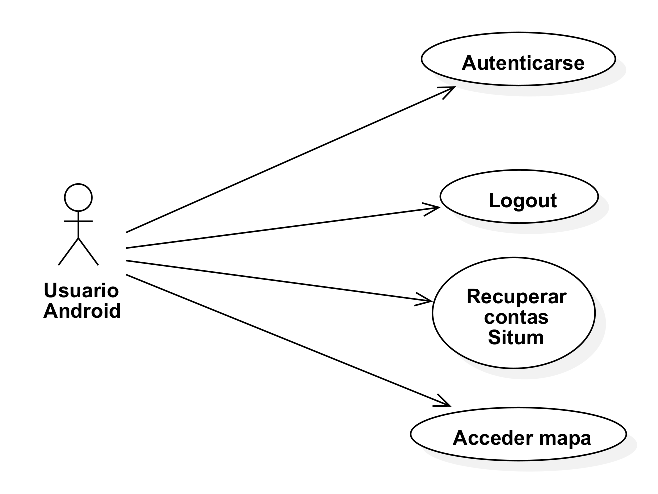
\includegraphics[width=0.5\textwidth]{figures/CasosUso/UsuarioAndroidPantallaInicial}
		\caption{Casos de uso do Usuario Android dentro da pantalla inicial.}
		\label{fig:cuUsuarioAndroidPantallaInicial}
	\end{center}
\end{figure}

\begin{itemize}
	\item Autenticarse: Este caso de uso é totalmente opcional xa que se permite usar o noso sistema de maneira anónima utilizando a aplicación. O usuario pode utilizar a súa conta de Google para identificarse dentro do noso sistema. Ao ser unha aplicación dirixida a Android non consideramos que sexa un impedimento para o uso xa que é preciso ter unha para utilizar o sistema operativo. Ver \ref{tab:cuAutenticar}.
	\item Logout: Permitiremos a opción de facer logout na aplicación para seleccionar outra conta distinta de Google ou acceder ao sistema de maneira anónima xa que non é impedimento non estar autenticado. Ver \ref{tab:cuLogout}.
	\item Recuperar contas Situm: No noso sistema permitimos o uso de varias contas de Situm, que son as que teñen permisos para localizarse dentro dos edificios. Non todas as contas de Situm estarán dispoñíbeis, poderanse restrinxir a nivel de usuario, facéndoas privadas. Debido que non é obrigatoria a autenticación para poder utilizar a aplicación, debemos permitir a existencia de contas que sexan públicas para os usuarios que non se autentiquen. Ver \ref{tab:cuRecuperarContasSitum}.
	\item Acceder mapa: Unha vez se escolla a conta de Situm poderase acceder ao mapa no que se visualizarán os edificios aos que ten acceso esa conta de Situm. Ver \ref{tab:cuAccederMapa}.
\end{itemize}

\subsubsection{Localización}
No seguinte punto descríbense as funcións relacionadas coa posición do usuario e a súa visualización dentro do mapa proporcionadas por Situm. Pódense observar na figura \ref{fig:cuUsuarioAndroidPrincipalLocalizacion}.

\begin{figure}[tbh]
	\begin{center}
		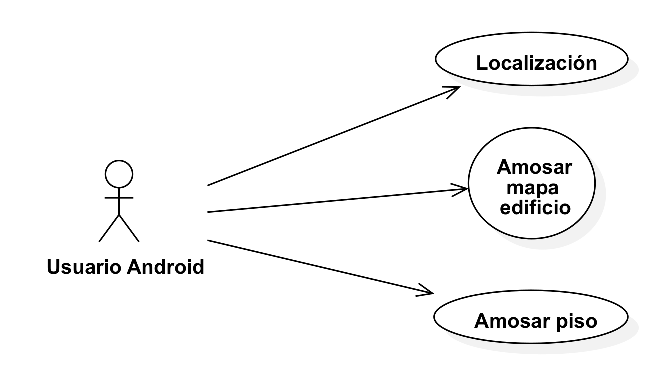
\includegraphics[width=0.5\textwidth]{figures/CasosUso/UsuarioAndroidLocalizacion}
		\caption{Casos de uso referentes á localización do Usuario Android.}
		\label{fig:cuUsuarioAndroidPrincipalLocalizacion}
	\end{center}
\end{figure}

\begin{itemize}
	\item Amosar mapa edificio: Se a conta de Situm seleccionada ten permisos para visualizar un edificio, a aplicación permitirá amosar os seus planos incluídos na plataforma de Situm. Esta acción realizarase sobre o mapa xeral que sirva de base para a aplicación Android e nas mesmas coordenadas onde se atopa realmente o edificio, superpoñendo os planos á súa situación real. Ver \ref{tab:cuAmosarMapaEdificio}.
	\item Amosar piso: Cando se teña un edificio seleccionado o cal se estea a amosar no mapa xeral, os usuarios terán a opción de cambiar o nivel que está a ser visualizado. Desta maneira poderase observar a estrutura de cada un dos pisos do edificio. Ver \ref{tab:cuCambiarPiso}.
	\item Localización: Se o usuario selecciona unha conta de Situm que ten permisos sobre certo edificio e se atopa fisicamente dentro del, a aplicación identifica esa localización con gran precisión e amosa un icono indicando esa posición. Ver \ref{tab:cuLocalizacion}.
\end{itemize}


\subsubsection{POIs e percorridos}
No seguinte punto descríbense as funcións relacionadas coa visualización dos puntos de interese (POIs) dun edificio e da conexión entre eles formando percorridos. Pódense observar na figura \ref{fig:cuUsuarioAndroidPrincipalPOIPercorrido}.

\begin{figure}[tbh]
	\begin{center}
		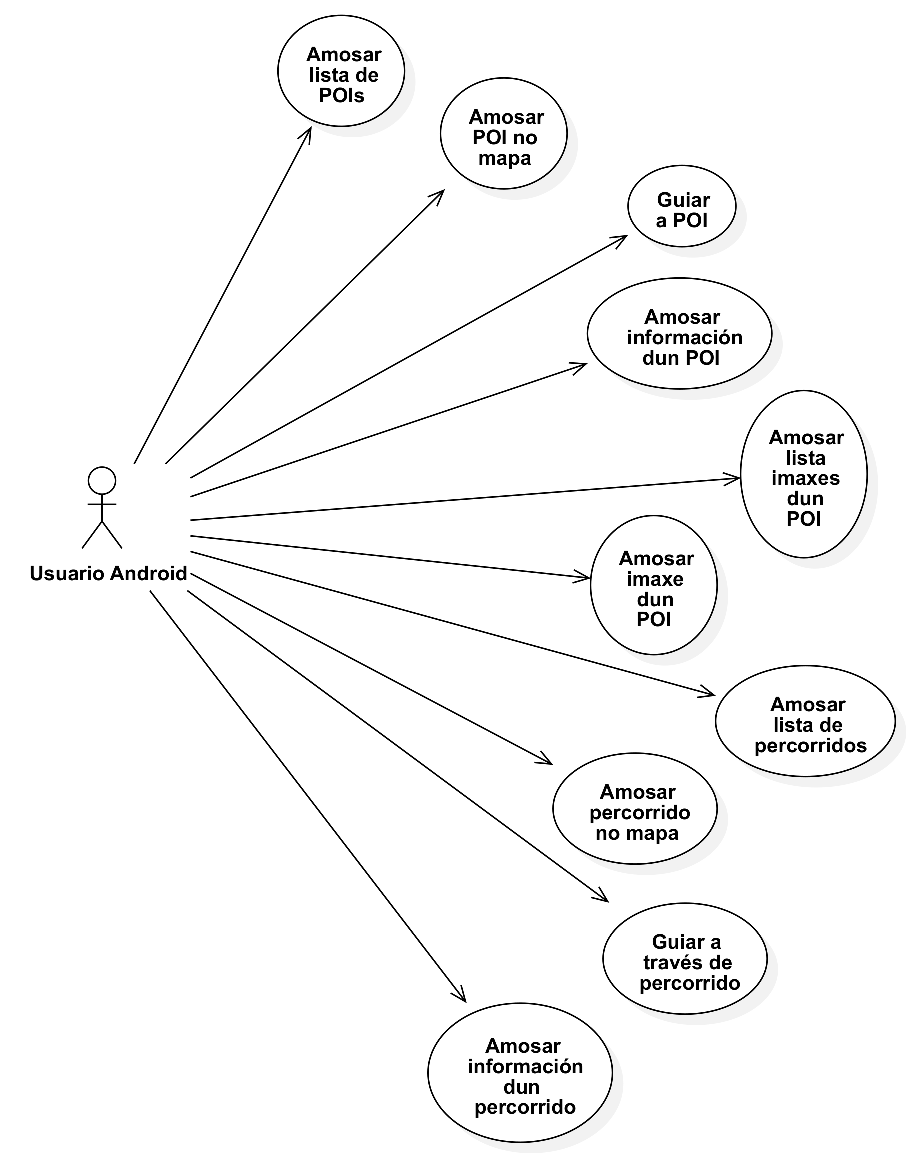
\includegraphics[width=0.7\textwidth]{figures/CasosUso/UsuarioAndroidPOIPercorrido}
		\caption{Casos de uso referentes á visualización de POIs e percorridos.}
		\label{fig:cuUsuarioAndroidPrincipalPOIPercorrido}
	\end{center}
\end{figure}

\begin{itemize}
	\item Amosar lista de POIs: Unha vez seleccionado un edificio, permítese a visualización dunha lista con todos os puntos de interese propios dese edificio. Ver \ref{tab:cuAmosarListaPOI}.
	\item Amosar POI no mapa: Seleccionando un POI da lista de puntos de interese situarase un marcador no mapa indicando a posición exacta dese punto. Ver \ref{tab:cuAmosarPOIMapa}.
	\item Guiar a POI: Habilítase a opción de guiado a calquera punto de interese existente no edificio a través das opcións dadas por Situm. As ordes proporcionadas permitirán avanzar pola ruta máis curta ata o punto desexado grazas á configuración de Situm. Ver \ref{tab:cuGuiarPOI}.
	\item Amosar información dun POI: Permite ao usuario visualizar todos os datos relativos a un punto de interese dun edificio gardada no noso sistema. Ver \ref{tab:cuAmosarPOI}.
	\item Amosar lista de imaxes dun POI: Unha vez seleccionado un punto de interese, permítese a visualización dunha lista con todas as imaxes dese POI. Ver \ref{tab:cuAmosarListaImaxePOI}.
	\item Amosar imaxe dun POI: De entre a lista de imaxes dun POI permitirase a selección dunha imaxe concreta para visualizala na pantalla.  Ver \ref{tab:cuAmosarImaxePOI}.
	\item Amosar lista de percorridos: Unha vez seleccionado un edificio, permítese a visualización dunha lista con todos os percorridos propios dese edificio. Ver \ref{tab:cuAmosarListaPercorrido}.
	\item Amosar percorrido no mapa: Seleccionando un percorrido da lista de percorridos situarase un marcador no mapa por cada punto de interese que compoña ese percorrido, uníndoos mediante liñas que mostren a dirección na cal se ten que realizar. Ver \ref{tab:cuAmosarPercorridoMapa}.
	\item Guiar a través dun percorrido: Habilítase a opción de guiado a través de calquera percorrido existente no edificio a grazas ás opcións dadas por Situm. Baséase no caso de uso "Guiar a POI", pero visualizarase no mapa o percorrido xa realizado e o que aínda non se realizou.. Ver \ref{tab:cuGuiarPercorrido}.
	\item Amosar información dun percorrido: Permite ao usuario visualizar toda a información relativa a un percorrido dun edificio gardada no noso sistema. Ver \ref{tab:cuAmosarPercorrido}.
\end{itemize}


\subsection{Xestor de contido}

A continuación exporemos os casos de uso do Xestor de contido. Para a realización destes casos de uso é preciso ter permiso de edición sobre o edificio en cuestión. A parte dos seus propios casos de uso tamén pode realizar todas as accións do Usuario Android.

\subsubsection{Puntos de interese}
No seguinte punto descríbense as funcións relacionadas coa creación e edición dos puntos de interese (POIs) dun edificio. Pódense observar na figura \ref{fig:cuXestorContidoPOI}.

\begin{figure}[tbh]
	\begin{center}
		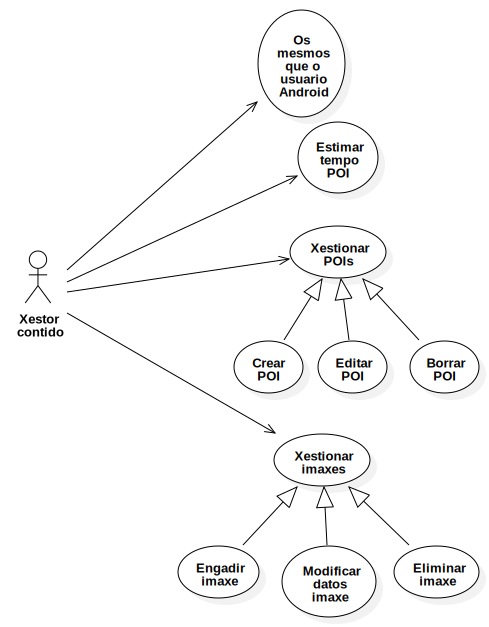
\includegraphics[width=0.6\textwidth]{figures/CasosUso/XestorContidoPoi}
		\caption{Casos de uso do Xestor de contido referentes aos POIs.}
		\label{fig:cuXestorContidoPOI}
	\end{center}
\end{figure}

\begin{itemize}
	\item Xestión de POIs - Creación: Unha vez seleccionado un edificio, permítese a creación dun punto de interese dentro dos diversos niveis nos que se pode dividir o edificio. Débese seleccionar a posición do novo punto e darlle un nome e unha descrición. Ver \ref{tab:cuCrearPOI}.
	\item Xestión de POIs - Edición: Seleccionando un POI da lista de puntos de interese poderase entrar nunha pantalla onde visualizar toda a súa información. Dende ese punto permítese a edición dos seus datos. Ver \ref{tab:cuModificarPOI}.
	\item Xestión de POIs - Borrado: Dende a mesma pantalla onde se visualiza e modifica a información dun POI débese permitir a eliminación dese punto, sempre que non estea incluído dentro dalgún percorrido. Ver \ref{tab:cuEliminarPOI}.
	\item Estimar tempo POI: Dende a mesma pantalla onde se visualiza e modifica a información dun POI débese permitir a estimación do tempo adicado a ese punto. Ver \ref{tab:cuEstimarTempoPOI}.
	\item Xestión de imaxes - Engadir: Existe a opción de incluír e asociar imaxes a distintos puntos de interese que permitan describir e completar a información dada sobre eles. Tamén será dende a pantalla de visualización dos datos dun POI onde se permitirá engadir imaxes, aportando información sobre elas. Ver \ref{tab:cuEngadirImaxe}.
	\item Xestión de imaxes - Modificar datos: Unha vez seleccionada unha imaxe dun punto de interese, permítese a modificación dos datos desa imaxe. Ver \ref{tab:cuModificarImaxe}.
	\item Xestión de imaxes - Eliminar: De entre a lista de imaxes dun POI permitirase a selección dunha imaxe concreta para eliminala do noso sistema. Ver \ref{tab:cuEliminarImaxe}.
\end{itemize}

\subsubsection{Percorridos}
Na figura \ref{fig:cuXestorContidoPercorrido} pódense observar todas as funcións que pode levar a cabo o actor relacionadas cos percorridos.

\begin{figure}[tbh]
	\begin{center}
		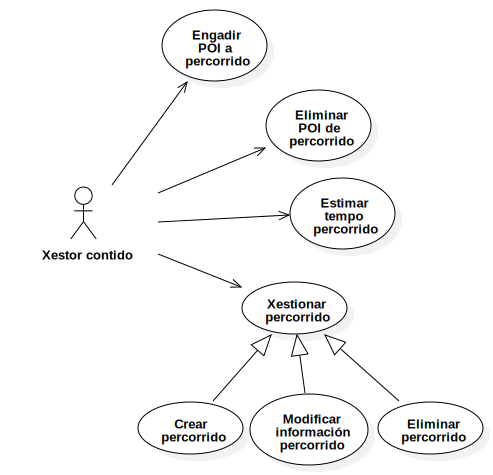
\includegraphics[width=0.6\textwidth]{figures/CasosUso/XestorContidoPercorrido}
		\caption{Casos de uso do Xestor de contido referentes aos percorridos.}
		\label{fig:cuXestorContidoPercorrido}
	\end{center}
\end{figure}

\begin{itemize}
	\item Xestión de percorridos - Creación: Permitiremos a creación de percorridos dende a pantalla principal, onde seleccionaremos todos os puntos de interese que o compoñan, paso previo á introdución da información asociada a ese percorrido dende a pantalla de inserción de datos. Non se poden repetir puntos de interese dentro do mesmo percorrido. O número mínimo será de 3 POIs. Ver \ref{tab:cuCrearPercorrido}.
	\item Xestión de percorridos - Modificar información: Unha vez seleccionado un percorrido dentro dun edificio, permítese a modificación dos seus datos. Ver \ref{tab:cuModificarPercorrido}.
	\item Xestión de percorridos - Eliminación: Unha vez seleccionado un percorrido dun edificio, permítese a eliminación do mesmo dende a pantalla de modificación da súa información. Ver \ref{tab:cuEliminarPercorrido}.
	\item Estimar tempo percorrido: Dende a mesma pantalla onde se visualiza e modifica a información dun percorrido débese permitir a estimación do tempo adicado a ese punto. Ver \ref{tab:cuEstimarTempoPercorrido}.
	\item Engadir POI a percorrido: Despois de seleccionar un percorrido disporase da posibilidade de engadir puntos de interese non incluídos xa dentro do mesmo. Esta inserción poderá ser ao inicio do percorrido, no final, ou tamén entre dous POIs xa incluídos. Ver \ref{tab:cuEngadirPOIPercorrido}.
	\item Eliminar POI de percorrido: Poderase escoller entre todos os POIs incluídos nun percorrido para a súa eliminación, sempre que non se deixe ao percorrido con menos de 3 POIs despois da eliminación. Ver \ref{tab:cuEliminarPOIPercorrido}.
\end{itemize}


\subsection{Administrador do sistema}
A continuación exporemos os casos de uso do Administrador do sistema. As accións levadas a cabo por este actor non se realizarán dende a aplicación, senón que haberá que utilizar algún xestor de base de datos. Na figura \ref{fig:cuAdministradorSistema} pódense observar estas accións.

\begin{figure}[tbh]
	\begin{center}
		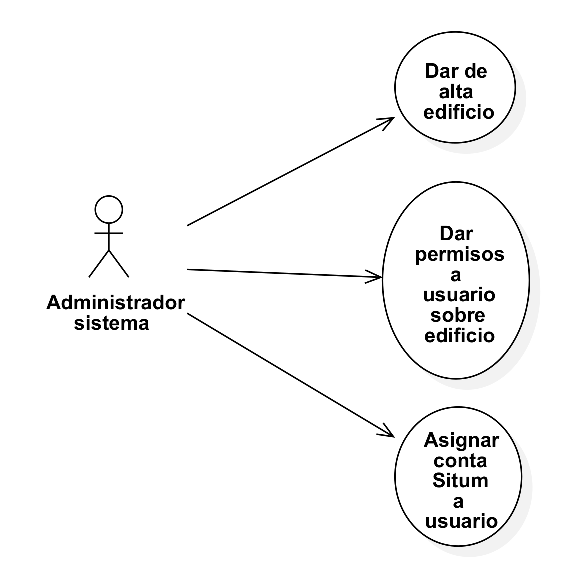
\includegraphics[width=0.5\textwidth]{figures/CasosUso/AdministradorSistema}
		\caption{Casos de uso do Xestor de contido referentes aos percorridos.}
		\label{fig:cuAdministradorSistema}
	\end{center}
\end{figure}

\begin{itemize}
	\item Dar de alta un edificio: Este será o primeiro paso para a introdución dun novo edificio dentro da nosa plataforma. Antes de poder engadir POIs e percorridos debemos inserir o edificio na base de datos, incluíndo información propia do sistema de Situm que nos permita ligar ambas plataformas. Ver \ref{tab:cuAltaEdificio}.
	\item Dar permisos a un usuario sobre algún edificio: Para permitir a creación de contido sobre os edificios débense dar permisos de xestor a algún usuario. Estes usuarios deben existir na base de datos, é dicir, debéronse autenticar nalgún momento na aplicación para poder ter os seus datos. Os permisos serán outorgados individualmente sobre cada edificio, para que un usuario non poida modificar todos os edificios dunha conta. Ver \ref{tab:cuDarPermisoUsuarioEdificio}.
	\item Asignar contas Situm a usuarios: Como non todos as contas de acceso ao sistema de Situm van estar visíbeis para calquera usuario que entre na aplicación, debemos asignar esas contas privadas a certos usuarios. Desta maneira, cando algún usuario acceda á aplicación, poderá ver tanto as contas de Situm públicas coma as privadas que estean asociadas ao seu usuario. Ver \ref{tab:cuAsignarContaSitumUsuario}.
\end{itemize}